
%------------------------------------------------------------------------
\section{Our Approach: GraphGround}
\begin{figure}
    \centering
    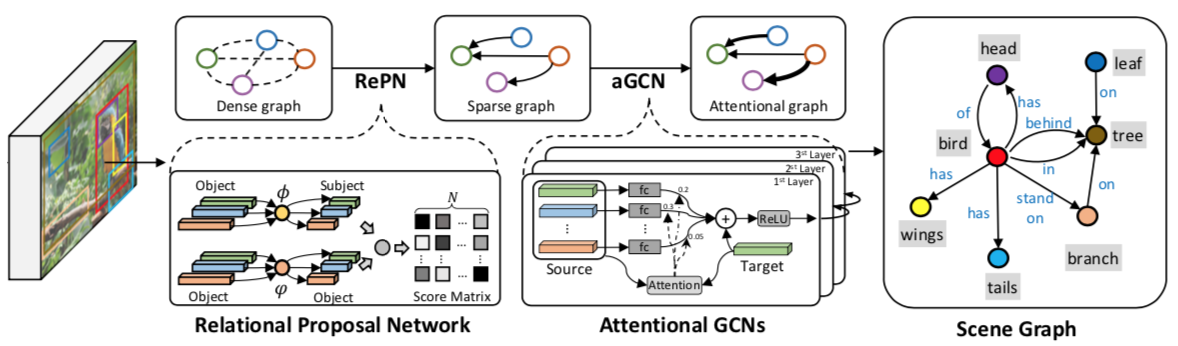
\includegraphics[width=0.5\textwidth]{latex/figures/graphrcnn_framework.png}
    \caption{Graph R-CNN Pipeline, illustration from \cite{yang2018graph}.}
    \label{fig:graphrcnn_framework}
\end{figure}

% Figure \ref{fig:graphrcnn_framework} shows the Graph R-CNN architecture.
We leverage the Graph R-CNN architecture for scene graph generation to learn a graph representation over the proposed regions. Our re-implementation follows the original work of \cite{yang2018graph} (see Fig. \ref{fig:graphrcnn_framework}) with minor modifications. Given an image $I$, we use Faster R-CNN \cite{ren2015faster} to generate bounding boxes $r_i = [x_i, y_i, w_i, h_i]$  around potential objects, along with their associated visual features $X_i \in \R^d$ and the distribution over label classes $P_i \in \R^c$. Here $i$ denotes the index of an arbitrary bounding box, $d$ is the visual feature dimension and $c$ is the number of object label classes. Then the RePN uses a learned asymmetric kernel function $\phi(P_i, P_j)$ to predict whether there should be a directed edge from $r_i$ to $r_j$, and incorrect edge assignments are penalized using a binary classification loss function. This gives us a graph with $n$ vertices (proposed bounding boxes) and $m$ edges (proposed relationships). The visual features $X_{ij}$ associated with the union of $r_i$ and $r_j$ are extracted as the initial edge features. Given the graph with its initial features $X_i$ and $X_{ij}$, an attentional GCN (aGCN) performs graph convolutions on the proposed graph to aggregate both node features and edge features.  The aGCN is a variant of GCN \cite{kipf2016semi} with the additional use of a weighted average during neighborhood aggregation based on attention scores. Finally, the node and the edge features are mapped to the node and edge label space respectively, where incorrect classifications are penalized via another loss function. 

For the downstream visual grounding task, our model is inspired by the supervised version of GroundeR \cite{rohrbach2016grounding}, where each query consists of a scene image and a phrase to be grounded, as well as the the groundtruth bounding box. We first extract the visual features of 100 proposed bounding boxes of the image and project them to a lower dimension $d$. The query phrase is encoded using a language model then fed into a LSTM, of which the hidden states are also projected to a $d$-dimensional latent space. After batch normalization, we sum the visual features with the hidden state of the LSTM, which then goes through an activation and finally projected onto the output label space, which consists of our bounding box proposals. This last layer is referred to as the ``attention"  \cite{rohrbach2016grounding} , which we can normalize using softmax and choose the index that gives rise to the highest probability as the predicted proposal index. The target proposal index corresponds to the proposal bounding box with the highest IoU (intersection over union) with the groundtruth bounding box (out of all proposed bounding boxes that has a $>$ 0.5 IoU with the groundtruth). This way, the grounding task simply boils down to an ordinary multi-class classification problem.

Instead of using visual features extracted from a pre-trained image classification network that neglects pairwise scene object interactions, we use the logits at the end of the aGCN of our Graph R-CNN model as the visual features. This way, the features have been optimized to preserve the pairwise relationship between scene objects, and thus provide a more comprehensive representation of the proposals to be grounded. Intuitively, suppose that there are two proposal bounding boxes that both capture ``hands" in a similar posture, but are from two different people. In this case, visual features from a generic image classification network would treat the two proposals independently, hence giving similar visual features due to their pixel-level similarity. However, visual features from the scene graph embeddings should ideally be much more different, as the relationship between scene objects are constraining the objects to be more distinguishable. Since the grounding benchmark dataset Flickr30k Entities \cite{plummer2015flickr30k} does not provide scene graph annotations, we use the Visual Genome dataset \cite{krishna2017visual} to pre-train our Graph R-CNN model, and then generate scene graphs on the Flickr30k Entities images to provide bounding box proposals as well as enhanced visual features. 
